\section{Linearization}\label{se:linearization}
To be able to obtain a MPC control algorithm the system needs to be transform into state space form. In this section it will be elaborated how this is obtained.


The continuity equation from section ??? and an equation to describe the flow knowing the height is used found in section ????. 
\begin{equation}\label{eq:linearization_Continuity}
\frac{\partial A(x,t)}{\partial t} + \frac{\partial Q(x,t)}{\partial x}=0
\end{equation}

\begin{equation}
	Q = f(h) = \left(0.46-0.5 \cdot cos\left(\pi \frac{h}{d}\right)+0.04\cdot cos\left(2\pi\frac{h}{d}\right)\right)Q_f
\end{equation}

Equation \ref{eq:linearization_Continuity} is expanded to the following:

\begin{equation}
	\frac{\partial A(h)}{\partial h}\frac{\partial h(x,t)}{\partial t} + \frac{\partial Q(h)}{\partial h}\frac{\partial h(x,t)}{\partial x}=0
\end{equation}

By applying the Preissmann scheme from section \ref{subse:preissmann_scheme} equation \ref{eq:preissmann_time_derivatie} and \ref{eq:preissmann_space_derivatie} on the partial derivate of h in terms of time and position, the following is obtained: 

\begin{equation}
\begin{aligned}
	&\frac{\partial A(x,t)}{\partial h} \left(\frac{1}{2}\frac{h_{j+1}^{i+1}-h_{j+1}^i}{\Delta t} +  \frac{1}{2} \frac{h_{j}^{i+1} - h_j^i}{\Delta t}\right) + \\ &\frac{\partial Q(x,t)}{\partial h}\left(\theta \frac{h_{j+1}^{i+1}-h_j^{i+1}}{\Delta x}+(1-\theta)\frac{h_{j+1}^i - h_j^i}{\Delta x}\right)=0
\end{aligned}
\end{equation}
This equation can be written on a matrix form:

\begin{equation}
\begin{aligned}
	&\begin{bmatrix}
		\underbrace{\frac{1}{2\Delta t}\frac{\partial A}{\partial h}-\frac{\theta}{\Delta x}\frac{\partial Q}{\partial h}}_{a}   \underbrace{\frac{1}{2\Delta t}\frac{\partial A}{\partial h}+\frac{\theta}{\Delta x}\frac{\partial Q}{\partial h}}_{b} 
	\end{bmatrix}
	\begin{bmatrix}
		h_{j}^{i+1} \\
		h_{j+1}^{i+1}
	\end{bmatrix}
	= \\ -
	&\begin{bmatrix}
		\underbrace{\frac{-1}{2\Delta t}\frac{\partial A}{\partial h}-\frac{(1-\theta)}{\Delta x}\frac{\partial Q}{\partial h}}_{c} & \underbrace{\frac{-1}{2\Delta t}\frac{\partial A}{\partial h}+\frac{\theta}{\Delta x}\frac{\partial Q}{\partial h}}_{d} 
	\end{bmatrix}
	\begin{bmatrix}
		h_{j}^{i} \\
		h_{j+1}^{i}
	\end{bmatrix}
	\end{aligned}
\end{equation}

We want the equation on the normal state space form.

\begin{equation}
	\dot{x} = Ax + Bu
\end{equation}
Where A is the system matrix, x is the state of the system, B is the input matrix and u is the input. 

\begin{equation}
\begin{aligned}
	   \underbrace{\begin{bmatrix}
	    	a & b \\
	    	  & \ddots  & \ddots \\
	    	  &  		& a  		&b\\
	          &  		&  			&  a\\
	   \end{bmatrix}}_{\xi}
	    \underbrace{\begin{bmatrix}
		h_{1}^{i+1} \\
		h_{2}^{i+1}\\
		\vdots		\\
		h_{m}^{i+1}\\
	\end{bmatrix}}_{\dot{x}}
	= -
	\underbrace{\begin{bmatrix}
	    	d &  \\
	    	c & d & \\
	    	  &	\ddots  & \ddots   \\
	    	  &   &  c &  d\\
	    \end{bmatrix}}_{A}
	    	\underbrace{\begin{bmatrix}
		h_{1}^{i} \\
		h_{2}^{i}\\
		\vdots		\\
		h_{m}^{i}\\
		\end{bmatrix}}_{x}
	+ \underbrace{\begin{bmatrix}
		c \\
		\vdots		\\
		0\\
		\end{bmatrix}}_{B}
		\underbrace{\begin{bmatrix}
		h_{0} \\
		\vdots		\\
		0\\
		\end{bmatrix}}_{u}
	\end{aligned}
\end{equation}
Where m denotes the channel pieces.  
To obtain a state space for the matrix to the left needs to inversed, thereby obtaining the following equation:

\begin{equation}
	\dot{x} = -\xi^{-1} (Ax+Bu)
\end{equation}



\begin{figure}[H]
 \centering
 % This file was created by matlab2tikz.
%
%The latest updates can be retrieved from
%  http://www.mathworks.com/matlabcentral/fileexchange/22022-matlab2tikz-matlab2tikz
%where you can also make suggestions and rate matlab2tikz.
%
\definecolor{mycolor1}{rgb}{0.00000,0.44700,0.74100}%
%
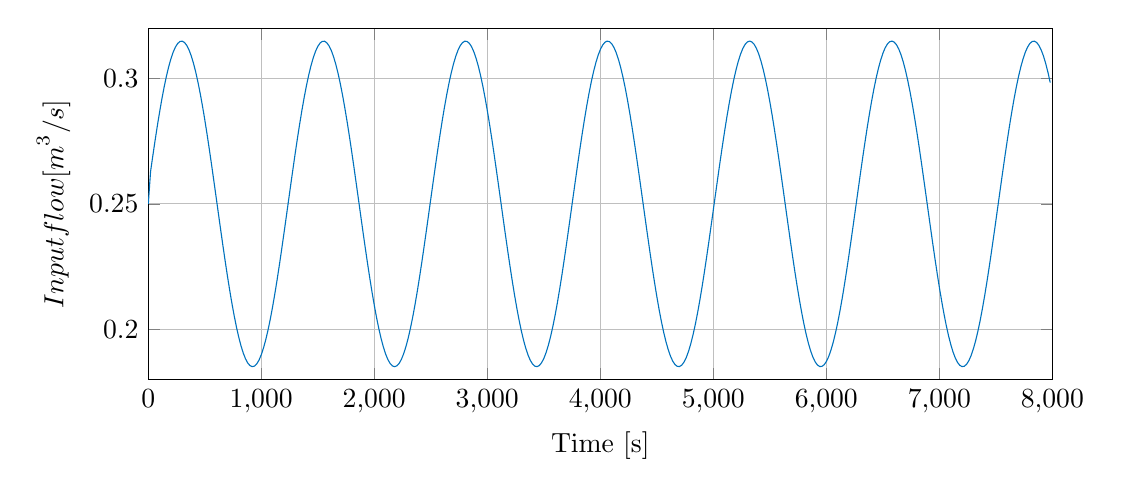
\begin{tikzpicture}

\begin{axis}[%
width=4.521in,
height=1.7566in,
at={(0.758in,0.481in)},
scale only axis,
xmin=0,
xmax=8000,
xlabel={Time [s]},
xmajorgrids,
ymin=0.18,
ymax=0.32,
ylabel={$\text{Input flow [m}^\text{3}\text{/s]}$},
ymajorgrids,
axis background/.style={fill=white}
]
\addplot [color=mycolor1,solid,forget plot]
  table[row sep=crcr]{%
1	0.250000001997809\\
21	0.262886754653035\\
41	0.269169019141146\\
61	0.275259753146396\\
81	0.281098100067933\\
101	0.286625725073218\\
121	0.291787397960388\\
141	0.296531545000176\\
161	0.300810764243567\\
181	0.304582299146404\\
201	0.307808465778641\\
221	0.310457029349718\\
241	0.31250152628793\\
261	0.313921528655692\\
281	0.314702848258737\\
301	0.314837678409859\\
321	0.314324671930759\\
341	0.313168954612597\\
361	0.311382074000788\\
381	0.308981884015741\\
401	0.305992366562389\\
421	0.302443391910922\\
441	0.298370420242923\\
461	0.293814147344954\\
481	0.288820097989707\\
501	0.283438171067526\\
521	0.27772214101319\\
541	0.271729120509533\\
561	0.265518989836398\\
581	0.259153798566676\\
601	0.25269714558748\\
621	0.246213543641094\\
641	0.239767774734971\\
661	0.233424242861334\\
681	0.227246330493771\\
701	0.221295765290512\\
721	0.215632003332074\\
741	0.210311635055753\\
761	0.205387819822688\\
781	0.20090975476709\\
801	0.196922183234743\\
821	0.193464947722282\\
841	0.190572591784138\\
861	0.188274014884759\\
881	0.186592183644715\\
901	0.185543902365817\\
921	0.185139645128088\\
941	0.185383451136218\\
961	0.186272884361165\\
981	0.187799057880153\\
1001	0.189946722671866\\
1021	0.192694419979629\\
1041	0.19601469572021\\
1061	0.199874374795948\\
1081	0.204234892569357\\
1101	0.209052680188242\\
1121	0.214279599911263\\
1141	0.219863426084337\\
1161	0.225748366962111\\
1181	0.231875622160638\\
1201	0.238183970171374\\
1221	0.244610380066258\\
1241	0.251090641281911\\
1261	0.257560005190354\\
1281	0.263953832045903\\
1301	0.270208236844133\\
1321	0.276260727639734\\
1341	0.282050829945362\\
1361	0.287520690972733\\
1381	0.292615657678558\\
1401	0.297284822839683\\
1421	0.30148153370124\\
1441	0.305163858115549\\
1461	0.308295003514275\\
1481	0.310843684527614\\
1501	0.312784435577363\\
1521	0.31409786532056\\
1541	0.314770850401372\\
1561	0.314796666575332\\
1581	0.314175055895763\\
1601	0.312912229291097\\
1621	0.311020804507335\\
1641	0.308519680035693\\
1661	0.30543384628513\\
1681	0.301794135886441\\
1701	0.297636915622801\\
1721	0.293003723064891\\
1741	0.287940851541218\\
1761	0.282498887590485\\
1781	0.276732205517613\\
1801	0.270698424103663\\
1821	0.26445783089802\\
1841	0.258072779845129\\
1861	0.251607068264493\\
1881	0.245125299408945\\
1901	0.238692236970304\\
1921	0.232372157981967\\
1941	0.226228210584045\\
1961	0.220321783068021\\
1981	0.214711890505228\\
2001	0.20945458508777\\
2021	0.204602396073545\\
2041	0.200203804931261\\
2061	0.196302760929632\\
2081	0.192938242010808\\
2101	0.190143865335664\\
2121	0.18794755139224\\
2141	0.186371245023454\\
2161	0.185430696161485\\
2181	0.185135302459658\\
2201	0.185488015394197\\
2221	0.186485310774052\\
2241	0.188117223953449\\
2261	0.190367449395338\\
2281	0.19321350359093\\
2301	0.196626949707483\\
2321	0.200573681719736\\
2341	0.205014265186038\\
2361	0.209904331264255\\
2381	0.215195020030576\\
2401	0.220833468671715\\
2421	0.226763339672675\\
2441	0.232925383722569\\
2461	0.23925803171415\\
2481	0.245698009921982\\
2501	0.252180972212586\\
2521	0.258642142969737\\
2541	0.265016964311009\\
2561	0.271241741128795\\
2581	0.277254277510769\\
2601	0.282994498180884\\
2621	0.288405048751668\\
2641	0.293431868790308\\
2661	0.298024731972623\\
2681	0.302137747927896\\
2701	0.305729820760282\\
2721	0.308765059665423\\
2741	0.311213137539494\\
2761	0.313049593997605\\
2781	0.314256079773878\\
2801	0.314820540061248\\
2821	0.31473733495911\\
2841	0.314007295825339\\
2861	0.312637716969642\\
2881	0.310642282771222\\
2901	0.308040930948987\\
2921	0.304859653350452\\
2941	0.301130236249792\\
2961	0.296889942749893\\
2981	0.292181140461754\\
3001	0.287050878181313\\
3021	0.281550415793439\\
3041	0.275734712100098\\
3061	0.26966187569018\\
3081	0.263392584337679\\
3101	0.256989478729437\\
3121	0.250516536580106\\
3141	0.244038433387972\\
3161	0.237619896218756\\
3181	0.231325056974165\\
3201	0.225216811607134\\
3221	0.219356191686253\\
3241	0.213801754588509\\
3261	0.208608998413328\\
3281	0.203829807463917\\
3301	0.199511933836451\\
3321	0.195698520296917\\
3341	0.192427669212855\\
3361	0.189732061847097\\
3381	0.187638631817393\\
3401	0.186168295984603\\
3421	0.18533574545834\\
3441	0.185149298808259\\
3461	0.185610818947655\\
3481	0.186715694519854\\
3501	0.188452885973362\\
3521	0.190805035865415\\
3541	0.193748642291808\\
3561	0.197254293710156\\
3581	0.201286962810301\\
3601	0.205806356495619\\
3621	0.210767318478317\\
3641	0.21612028046614\\
3661	0.221811757432362\\
3681	0.227784882020486\\
3701	0.233979972744082\\
3721	0.240335130304463\\
3741	0.246786856068022\\
3761	0.253270686523587\\
3781	0.259721837380514\\
3801	0.26607585087191\\
3821	0.272269239795324\\
3841	0.278240121855897\\
3861	0.28392883797379\\
3881	0.289278548377994\\
3901	0.294235800530528\\
3921	0.298751063206534\\
3941	0.3027792213939\\
3961	0.306280027067552\\
3981	0.309218501334409\\
4001	0.311565283930928\\
4021	0.313296926581148\\
4041	0.314396127284113\\
4061	0.314851903189745\\
4081	0.314659700335857\\
4101	0.313821439149829\\
4121	0.312345495260341\\
4141	0.310246615810853\\
4161	0.307545772111028\\
4181	0.304269950098335\\
4201	0.300451880703481\\
4221	0.296129712813773\\
4241	0.291346632102048\\
4261	0.286150429529699\\
4281	0.280593023835195\\
4301	0.2747299427792\\
4321	0.268619768329549\\
4341	0.262323551329587\\
4361	0.255904201498327\\
4381	0.249425858857326\\
4401	0.242953252864798\\
4421	0.236551055660262\\
4441	0.230283235881899\\
4461	0.224212419513071\\
4481	0.218399264144189\\
4501	0.212901852902125\\
4521	0.207775114102807\\
4541	0.203070272425644\\
4561	0.19883433709346\\
4581	0.19510963217188\\
4601	0.191933373681257\\
4621	0.189337297746497\\
4641	0.187347343500193\\
4661	0.185983393907381\\
4681	0.185259077101532\\
4701	0.185181630216741\\
4721	0.185751827076682\\
4741	0.186963970462812\\
4761	0.188805949039098\\
4781	0.191259358364483\\
4801	0.194299684783977\\
4821	0.197896550360995\\
4841	0.202014016403656\\
4861	0.206610942552316\\
4881	0.211641397840439\\
4901	0.217055119621635\\
4921	0.222798015777402\\
4941	0.228812705187703\\
4961	0.235039091064141\\
4981	0.241414961417209\\
5001	0.247876610657921\\
5021	0.254359476123001\\
5041	0.260798783163673\\
5061	0.267130192352538\\
5081	0.273290442341866\\
5101	0.279217981950073\\
5121	0.284853585160777\\
5141	0.290140942889579\\
5161	0.295027225605822\\
5181	0.299463611187795\\
5201	0.303405772737236\\
5221	0.30681432147905\\
5241	0.309655200320925\\
5261	0.311900024140542\\
5281	0.313526363400335\\
5301	0.314517968256018\\
5321	0.314864930919653\\
5341	0.314563784654995\\
5361	0.313617538415976\\
5381	0.312035646782229\\
5401	0.309833915492053\\
5421	0.307034343516705\\
5441	0.303664903253947\\
5461	0.299759261037095\\
5481	0.295356440752147\\
5501	0.290500433924011\\
5521	0.285239760167731\\
5541	0.279626982396533\\
5561	0.273718181630568\\
5581	0.267572396653901\\
5601	0.261251034118491\\
5621	0.254817254989228\\
5641	0.248335343460447\\
5661	0.241870064649509\\
5681	0.235486017485154\\
5701	0.229246989256365\\
5721	0.223215318270854\\
5741	0.217451270991304\\
5761	0.21201243987279\\
5781	0.206953167918012\\
5801	0.202324005699967\\
5821	0.198171206277341\\
5841	0.194536263049232\\
5861	0.191455495166822\\
5881	0.188959684644427\\
5901	0.187073768795781\\
5921	0.185816591068641\\
5941	0.185200712767292\\
5961	0.185232287544136\\
5981	0.185910999914442\\
6001	0.187230068408557\\
6021	0.189176313330114\\
6041	0.191730288443201\\
6061	0.194866475272719\\
6081	0.198553538076553\\
6101	0.202754636941948\\
6121	0.20742779587774\\
6141	0.212526322224584\\
6161	0.21799927319257\\
6181	0.223791964864743\\
6201	0.229846518580725\\
6221	0.236102439241154\\
6241	0.242497219754725\\
6261	0.248966965588378\\
6281	0.255447033180357\\
6301	0.26187267583731\\
6321	0.268179690661843\\
6341	0.274305060046651\\
6361	0.280187581325618\\
6381	0.28576847829063\\
6401	0.290991988464009\\
6421	0.295805920258768\\
6441	0.300162174459687\\
6461	0.304017224814776\\
6481	0.307332552935198\\
6501	0.310075033158275\\
6521	0.312217263528162\\
6541	0.31373783958713\\
6561	0.314621568241833\\
6581	0.314859619567676\\
6601	0.3144496150345\\
6621	0.313395651272071\\
6641	0.311708259137909\\
6661	0.309404298496441\\
6681	0.306506789760808\\
6701	0.303044683880508\\
6721	0.299052573073076\\
6741	0.294570345190085\\
6761	0.289642785170914\\
6781	0.284319127566438\\
6801	0.278652564603675\\
6821	0.272699714706633\\
6841	0.266520056783731\\
6861	0.260175335934213\\
6881	0.25372894651152\\
6901	0.247245298707871\\
6921	0.240789174988911\\
6941	0.234425082808731\\
6961	0.228216610072703\\
6981	0.222225789788159\\
7001	0.216512480251079\\
7021	0.21113376696179\\
7041	0.206143392245513\\
7061	0.201591218276812\\
7081	0.197522728873234\\
7101	0.193978575036038\\
7121	0.190994168778821\\
7141	0.188599329302394\\
7161	0.186817985051175\\
7181	0.185667934628089\\
7201	0.185160668956807\\
7221	0.185301256468237\\
7241	0.186088292458437\\
7261	0.187513913123951\\
7281	0.189563874134338\\
7301	0.19221769295681\\
7321	0.195448853510927\\
7341	0.199225071108512\\
7361	0.203508615031583\\
7381	0.208256685525211\\
7401	0.213421841438528\\
7421	0.21895247424102\\
7441	0.22479332367791\\
7461	0.230886029912352\\
7481	0.237169716637634\\
7501	0.243581599333105\\
7521	0.250057612586361\\
7541	0.256533050213659\\
7561	0.262943211782723\\
7581	0.269224049078072\\
7601	0.275312806049621\\
7621	0.281148645850384\\
7641	0.286673258698145\\
7661	0.291831444487524\\
7681	0.296571664331181\\
7701	0.300846555519349\\
7721	0.304613404752365\\
7741	0.307834574917848\\
7761	0.310477881148283\\
7781	0.312516912401574\\
7801	0.313931295351455\\
7821	0.314706897951021\\
7841	0.31483597063548\\
7861	0.314317223753232\\
7881	0.313155840451651\\
7901	0.311363424888784\\
7921	0.308957886288441\\
7941	0.305963259997152\\
7961	0.302409467330926\\
7981	0.298332016611358\\
};
\end{axis}
\end{tikzpicture}%
\caption{Input height for the simulation.}
\label{fig:height_input_for_comparision}
\end{figure}

\begin{figure}[H]
 \centering
 % This file was created by matlab2tikz.
%
%The latest updates can be retrieved from
%  http://www.mathworks.com/matlabcentral/fileexchange/22022-matlab2tikz-matlab2tikz
%where you can also make suggestions and rate matlab2tikz.
%
\definecolor{mycolor1}{rgb}{0.00000,0.44700,0.74100}%
\definecolor{mycolor2}{rgb}{0.85000,0.32500,0.09800}%
%
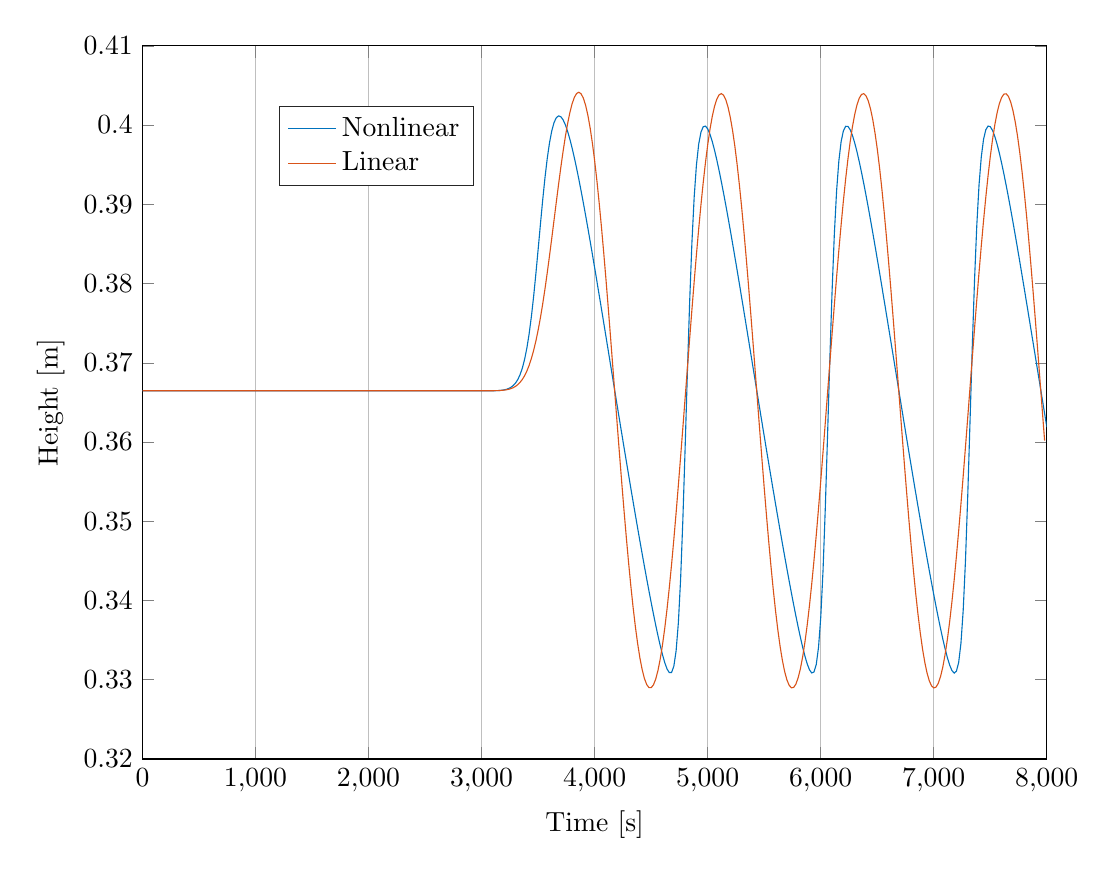
\begin{tikzpicture}

\begin{axis}[%
width=4.521in,
height=3.566in,
at={(0.758in,0.481in)},
scale only axis,
xmin=1,
xmajorgrids,
xmax=8000,
xlabel={Time [s]},
ymin=0.32,
ymax=0.41,
ylabel={Height [m]},
axis background/.style={fill=white},
legend style={at={(0.151,0.803)},anchor=south west,legend cell align=left,align=left,draw=white!15!black}
]
\addplot [color=mycolor1,solid]
  table[row sep=crcr]{%
1	0.366466627539343\\
21	0.366466665471691\\
41	0.366466692465574\\
61	0.366466711161801\\
81	0.366466723804557\\
101	0.366466732185832\\
121	0.36646673764237\\
141	0.366466741130459\\
161	0.366466743316878\\
181	0.366466744658372\\
201	0.366466745462716\\
221	0.366466745933408\\
241	0.366466746202002\\
261	0.366466746351381\\
281	0.366466746432328\\
301	0.366466746475058\\
321	0.366466746497021\\
341	0.366466746507986\\
361	0.366466746513251\\
381	0.366466746515595\\
401	0.366466746516464\\
421	0.366466746516784\\
441	0.366466746517842\\
461	0.366466746523015\\
481	0.366466746542095\\
501	0.366466746602594\\
521	0.366466746778925\\
541	0.366466747266689\\
561	0.366466748569185\\
581	0.366466751960835\\
601	0.366466760628919\\
621	0.366466782467414\\
641	0.366466824991748\\
661	0.366466877551302\\
681	0.366466909012503\\
701	0.366466897208555\\
721	0.366466852534906\\
741	0.366466804147601\\
761	0.366466772150041\\
781	0.366466758747709\\
801	0.366466757277496\\
821	0.366466761510951\\
841	0.366466768027839\\
861	0.366466774891905\\
881	0.366466780360355\\
901	0.366466782584759\\
921	0.366466779950668\\
941	0.366466771652426\\
961	0.366466758289697\\
981	0.366466742200663\\
1001	0.366466727015492\\
1021	0.366466716248985\\
1041	0.366466711712184\\
1061	0.36646671292079\\
1081	0.366466717849068\\
1101	0.366466724270585\\
1121	0.366466730692934\\
1141	0.366466736503687\\
1161	0.366466741612614\\
1181	0.366466746070639\\
1201	0.366466749918425\\
1221	0.366466753212207\\
1241	0.366466756057859\\
1261	0.366466758568098\\
1281	0.366466760782904\\
1301	0.366466762630246\\
1321	0.366466763956583\\
1341	0.366466764600551\\
1361	0.366466764466437\\
1381	0.366466763568626\\
1401	0.366466762037936\\
1421	0.366466760093622\\
1441	0.366466757992639\\
1461	0.366466755973411\\
1481	0.366466754212242\\
1501	0.366466752803997\\
1521	0.366466751767025\\
1541	0.366466751062805\\
1561	0.366466750618922\\
1581	0.366466750348598\\
1601	0.366466750165625\\
1621	0.366466749995936\\
1641	0.366466749786227\\
1661	0.3664667495087\\
1681	0.366466749160881\\
1701	0.366466748760672\\
1721	0.366466748338205\\
1741	0.366466747926767\\
1761	0.366466747555017\\
1781	0.366466747241989\\
1801	0.366466746995384\\
1821	0.366466746812749\\
1841	0.366466746684462\\
1861	0.366466746597258\\
1881	0.366466746537244\\
1901	0.366466746491858\\
1921	0.366466746450686\\
1941	0.366466746405459\\
1961	0.366466746349626\\
1981	0.366466746277887\\
2001	0.366466746185904\\
2021	0.366466746070288\\
2041	0.366466745928832\\
2061	0.366466745760932\\
2081	0.366466745568062\\
2101	0.366466745354198\\
2121	0.366466745126059\\
2141	0.366466744893064\\
2161	0.366466744666916\\
2181	0.366466744460798\\
2201	0.366466744288228\\
2221	0.366466744161677\\
2241	0.366466744091142\\
2261	0.366466744082878\\
2281	0.366466744138518\\
2301	0.366466744254728\\
2321	0.366466744423502\\
2341	0.36646674463305\\
2361	0.36646674486915\\
2381	0.366466745116762\\
2401	0.366466745361616\\
2421	0.366466745591559\\
2441	0.366466745797464\\
2461	0.366466745973624\\
2481	0.366466746117661\\
2501	0.366466746230052\\
2521	0.366466746313472\\
2541	0.366466746372187\\
2561	0.366466746411741\\
2581	0.366466746439263\\
2601	0.366466746464757\\
2621	0.366466746503873\\
2641	0.366466746582789\\
2661	0.366466746746095\\
2681	0.366466747069193\\
2701	0.36646674767828\\
2721	0.366466748783901\\
2741	0.366466750739029\\
2761	0.366466754138687\\
2781	0.366466759982299\\
2801	0.36646676991917\\
2821	0.366466786593398\\
2841	0.366466814088952\\
2861	0.36646685843496\\
2881	0.366466928083948\\
2901	0.366467034252727\\
2921	0.366467190986076\\
2941	0.366467414840061\\
2961	0.366467724280932\\
2981	0.366468138783252\\
3001	0.366468676751559\\
3021	0.366469356580593\\
3041	0.366470160960045\\
3061	0.366470781403547\\
3081	0.366471022304454\\
3101	0.366471811024978\\
3121	0.366476427538425\\
3141	0.366487208981108\\
3161	0.366506895988427\\
3181	0.366538154958313\\
3201	0.366586229651467\\
3221	0.366657715979119\\
3241	0.366763499523946\\
3261	0.366917391782519\\
3281	0.367139043129368\\
3301	0.367454993617361\\
3321	0.367897574460509\\
3341	0.36850855187551\\
3361	0.369337832554681\\
3381	0.37043866992242\\
3401	0.371865159415155\\
3421	0.373661877605495\\
3441	0.375850343116391\\
3461	0.378414236067563\\
3481	0.381291378533925\\
3501	0.384372804695217\\
3521	0.387512844594873\\
3541	0.3905512657543\\
3561	0.393339024106083\\
3581	0.395760573204265\\
3601	0.397742212920716\\
3621	0.399253919158054\\
3641	0.400302489298008\\
3661	0.400921093207355\\
3681	0.401154805407434\\
3701	0.401054639418849\\
3721	0.400670054854328\\
3741	0.400044850827336\\
3761	0.399219931578186\\
3781	0.398231007240009\\
3801	0.397106391211165\\
3821	0.395869603122493\\
3841	0.394540406299105\\
3861	0.393135051133942\\
3881	0.391665292279339\\
3901	0.390140640134986\\
3921	0.388569371321836\\
3941	0.386958604443187\\
3961	0.38531471749247\\
3981	0.383643494314967\\
4001	0.381950063243732\\
4021	0.380238783307623\\
4041	0.378513224443925\\
4061	0.376776293633958\\
4081	0.375030462811205\\
4101	0.373278012271646\\
4121	0.371521207603475\\
4141	0.369762211219868\\
4161	0.368003981050243\\
4181	0.366248027876198\\
4201	0.364495589895054\\
4221	0.36274817837337\\
4241	0.361007152561846\\
4261	0.359273873239861\\
4281	0.357549838340364\\
4301	0.355836692094989\\
4321	0.354136130444112\\
4341	0.352449809744458\\
4361	0.350779359466021\\
4381	0.349126509850378\\
4401	0.347493244675979\\
4421	0.345881887104931\\
4441	0.344295128405862\\
4461	0.342736107800051\\
4481	0.341208644935977\\
4501	0.339717633803796\\
4521	0.33826955870226\\
4541	0.336873179515492\\
4561	0.335540622633128\\
4581	0.334289313421881\\
4601	0.333145351925141\\
4621	0.332149220420964\\
4641	0.331364845137868\\
4661	0.330898154725945\\
4681	0.330920611138669\\
4701	0.331701861406759\\
4721	0.333627016627402\\
4741	0.337160391967049\\
4761	0.342687389504208\\
4781	0.350238925379372\\
4801	0.359278979022061\\
4821	0.368794883507088\\
4841	0.37768617476616\\
4861	0.385162896231032\\
4881	0.390901512494647\\
4901	0.394957571487544\\
4921	0.397587637909411\\
4941	0.399103627806496\\
4961	0.399788283600559\\
4981	0.399867543422794\\
5001	0.39950909035249\\
5021	0.398831004158808\\
5041	0.397918849649403\\
5061	0.396831762165564\\
5081	0.395610614486114\\
5101	0.394285153457823\\
5121	0.3928774871264\\
5141	0.391402867141369\\
5161	0.389872855411301\\
5181	0.388296811340508\\
5201	0.386682245098759\\
5221	0.385035455056554\\
5241	0.383361890492746\\
5261	0.381666299510196\\
5281	0.379952784260602\\
5301	0.378224870546435\\
5321	0.376485619899744\\
5341	0.374737747980308\\
5361	0.372983713654822\\
5381	0.371225798099233\\
5401	0.36946610982738\\
5421	0.367707346012034\\
5441	0.36595097244915\\
5461	0.364198476560114\\
5481	0.362451679502103\\
5501	0.360712151476488\\
5521	0.358981259374727\\
5541	0.357260283676455\\
5561	0.355550513137554\\
5581	0.353853314735917\\
5601	0.352170204157126\\
5621	0.350502906793907\\
5641	0.348853389344001\\
5661	0.347223875832671\\
5681	0.345616877505002\\
5701	0.344035250737081\\
5721	0.342482293026944\\
5741	0.340961912112083\\
5761	0.339478946792838\\
5781	0.338039744245102\\
5801	0.336653094188786\\
5821	0.335331662543733\\
5841	0.334094230460581\\
5861	0.332969329119605\\
5881	0.33200112977471\\
5901	0.331259545943237\\
5921	0.330859362295213\\
5941	0.330986746043631\\
5961	0.331929449934038\\
5981	0.334090502395966\\
6001	0.337936144363351\\
6021	0.343813694095991\\
6041	0.351668387281232\\
6061	0.360868048451852\\
6081	0.370353489513562\\
6101	0.37905274639098\\
6121	0.386250226872436\\
6141	0.391696415926776\\
6161	0.395492912117389\\
6181	0.39791438712643\\
6201	0.399272584189829\\
6221	0.399842045257527\\
6241	0.399838368584545\\
6261	0.399420391023125\\
6281	0.398698828491274\\
6301	0.397753915648429\\
6321	0.39664151960812\\
6341	0.395400219691452\\
6361	0.394058510709846\\
6381	0.392637268257605\\
6401	0.391151007525382\\
6421	0.389610922960775\\
6441	0.388026068082844\\
6461	0.386403786553424\\
6481	0.384750354678642\\
6501	0.383071309587512\\
6521	0.381371532327119\\
6541	0.37965522446482\\
6561	0.377925912612961\\
6581	0.37618653308801\\
6601	0.374439566745701\\
6621	0.372687159542499\\
6641	0.37093123369377\\
6661	0.369173762904317\\
6681	0.367417034013407\\
6701	0.365662198103127\\
6721	0.36391058042425\\
6741	0.362163892089778\\
6761	0.360423754996183\\
6781	0.358691793324237\\
6801	0.356969726303292\\
6821	0.355259390732162\\
6841	0.35356268781958\\
6861	0.351881499371196\\
6881	0.350217628278927\\
6901	0.348572810116784\\
6921	0.346948821893045\\
6941	0.345347668357579\\
6961	0.343771796843851\\
6981	0.342224323474826\\
7001	0.340709306127834\\
7021	0.339232116288827\\
7041	0.337799965520416\\
7061	0.336422693537365\\
7081	0.335114077562667\\
7101	0.333894157530986\\
7121	0.332793331053009\\
7141	0.331858832042384\\
7161	0.331166560746507\\
7181	0.330841014355229\\
7201	0.331083601276122\\
7221	0.332200931959585\\
7241	0.334612787291948\\
7261	0.33878182052881\\
7281	0.345008300801698\\
7301	0.353146585755168\\
7321	0.362473141745206\\
7341	0.371894864520334\\
7361	0.380379351083128\\
7381	0.387288734981073\\
7401	0.392443966115048\\
7421	0.395987436828022\\
7441	0.398207733177049\\
7461	0.399413773339763\\
7481	0.39987142748879\\
7501	0.399786479958598\\
7521	0.399309478906048\\
7541	0.398545717854504\\
7561	0.397571286774141\\
7581	0.396438242170758\\
7601	0.395181986798585\\
7621	0.393829305856599\\
7641	0.392398715789982\\
7661	0.390903890750215\\
7681	0.389355936704368\\
7701	0.387763859127099\\
7721	0.38613514005755\\
7741	0.384476100964206\\
7761	0.38279213085877\\
7781	0.381087856541197\\
7801	0.379367293514824\\
7821	0.37763396175543\\
7841	0.375890946504859\\
7861	0.374140924826797\\
7881	0.372386196920327\\
7901	0.370628746234173\\
7921	0.368870823401302\\
7941	0.367114475123368\\
7961	0.365360770569571\\
7981	0.363611061848541\\
8001	0.361866947544438\\
};
\addlegendentry{Nonlinear};

\addplot [color=mycolor2,solid]
  table[row sep=crcr]{%
1	0.366466627539343\\
21	0.366466627539343\\
41	0.366466627539343\\
61	0.366466627539343\\
81	0.366466627539343\\
101	0.366466627539343\\
121	0.366466627539343\\
141	0.366466627539343\\
161	0.366466627539343\\
181	0.366466627539343\\
201	0.366466627539343\\
221	0.366466627539343\\
241	0.366466627539343\\
261	0.366466627539343\\
281	0.366466627539343\\
301	0.366466627539343\\
321	0.366466627539343\\
341	0.366466627539343\\
361	0.366466627539343\\
381	0.366466627539343\\
401	0.366466627539343\\
421	0.366466627539343\\
441	0.366466627539343\\
461	0.366466627539343\\
481	0.366466627539343\\
501	0.366466627539343\\
521	0.366466627539343\\
541	0.366466627539343\\
561	0.366466627539343\\
581	0.366466627539343\\
601	0.366466627539343\\
621	0.366466627539343\\
641	0.366466627539343\\
661	0.366466627539343\\
681	0.366466627539343\\
701	0.366466627539343\\
721	0.366466627539343\\
741	0.366466627539343\\
761	0.366466627539343\\
781	0.366466627539343\\
801	0.366466627539343\\
821	0.366466627539343\\
841	0.366466627539343\\
861	0.366466627539343\\
881	0.366466627539343\\
901	0.366466627539343\\
921	0.366466627539343\\
941	0.366466627539343\\
961	0.366466627539343\\
981	0.366466627539343\\
1001	0.366466627539343\\
1021	0.366466627539343\\
1041	0.366466627539343\\
1061	0.366466627539343\\
1081	0.366466627539343\\
1101	0.366466627539343\\
1121	0.366466627539343\\
1141	0.366466627539343\\
1161	0.366466627539343\\
1181	0.366466627539343\\
1201	0.366466627539343\\
1221	0.366466627539343\\
1241	0.366466627539343\\
1261	0.366466627539343\\
1281	0.366466627539343\\
1301	0.366466627539343\\
1321	0.366466627539343\\
1341	0.366466627539343\\
1361	0.366466627539343\\
1381	0.366466627539343\\
1401	0.366466627539343\\
1421	0.366466627539343\\
1441	0.366466627539343\\
1461	0.366466627539343\\
1481	0.366466627539343\\
1501	0.366466627539343\\
1521	0.366466627539343\\
1541	0.366466627539343\\
1561	0.366466627539343\\
1581	0.366466627539343\\
1601	0.366466627539343\\
1621	0.366466627539343\\
1641	0.366466627539343\\
1661	0.366466627539343\\
1681	0.366466627539343\\
1701	0.366466627539343\\
1721	0.366466627539343\\
1741	0.366466627539343\\
1761	0.366466627539343\\
1781	0.366466627539343\\
1801	0.366466627539343\\
1821	0.366466627539343\\
1841	0.366466627539343\\
1861	0.366466627539343\\
1881	0.366466627539343\\
1901	0.366466627539343\\
1921	0.366466627539343\\
1941	0.366466627539343\\
1961	0.366466627539343\\
1981	0.366466627539343\\
2001	0.366466627539343\\
2021	0.366466627539343\\
2041	0.366466627539343\\
2061	0.366466627539343\\
2081	0.366466627539343\\
2101	0.366466627539343\\
2121	0.366466627539343\\
2141	0.366466627539343\\
2161	0.366466627539343\\
2181	0.366466627539343\\
2201	0.366466627539343\\
2221	0.366466627539343\\
2241	0.366466627539343\\
2261	0.366466627539343\\
2281	0.366466627539343\\
2301	0.366466627539343\\
2321	0.366466627539343\\
2341	0.366466627539343\\
2361	0.366466627539343\\
2381	0.366466627539343\\
2401	0.366466627539343\\
2421	0.366466627539343\\
2441	0.366466627539343\\
2461	0.366466627539343\\
2481	0.366466627539343\\
2501	0.366466627539344\\
2521	0.366466627539346\\
2541	0.366466627539352\\
2561	0.366466627539367\\
2581	0.366466627539406\\
2601	0.366466627539506\\
2621	0.366466627539753\\
2641	0.366466627540356\\
2661	0.366466627541801\\
2681	0.366466627545203\\
2701	0.36646662755307\\
2721	0.366466627570933\\
2741	0.366466627610775\\
2761	0.36646662769805\\
2781	0.366466627885832\\
2801	0.366466628282679\\
2821	0.366466629106458\\
2841	0.366466630786123\\
2861	0.366466634150207\\
2881	0.366466640768553\\
2901	0.366466653558754\\
2921	0.366466677839224\\
2941	0.366466723118069\\
2961	0.366466806064708\\
2981	0.36646695533534\\
3001	0.366467219229196\\
3021	0.366467677551623\\
3041	0.366468459553763\\
3061	0.366469770390096\\
3081	0.366471929138866\\
3101	0.366475421982078\\
3121	0.366480974508741\\
3141	0.366489647104487\\
3161	0.366502956796009\\
3181	0.366523027482528\\
3201	0.36655276798044\\
3221	0.366596073581188\\
3241	0.366658041875905\\
3261	0.366745187657059\\
3281	0.366865635273379\\
3301	0.36702926070058\\
3321	0.367247750875542\\
3341	0.367534545762865\\
3361	0.367904630390547\\
3381	0.368374150646985\\
3401	0.368959838382449\\
3421	0.369678247951269\\
3441	0.370544826519821\\
3461	0.371572862132087\\
3481	0.372772373883958\\
3501	0.374149024538009\\
3521	0.375703144660012\\
3541	0.377428956784265\\
3561	0.379314077344984\\
3581	0.38133935376884\\
3601	0.38347906633576\\
3621	0.385701492533075\\
3641	0.387969799702821\\
3661	0.390243203893882\\
3681	0.392478312407949\\
3701	0.394630556796896\\
3721	0.396655622738953\\
3741	0.398510792465058\\
3761	0.400156132117748\\
3781	0.401555477678416\\
3801	0.402677195711344\\
3821	0.403494716236732\\
3841	0.403986852338963\\
3861	0.404137933333533\\
3881	0.403937785095086\\
3901	0.403381592938361\\
3921	0.402469680258693\\
3941	0.401207231276515\\
3961	0.399603980007785\\
3981	0.397673881135668\\
4001	0.395434772626878\\
4021	0.392908035224715\\
4041	0.390118250560682\\
4061	0.387092857521657\\
4081	0.383861805500206\\
4101	0.380457202977927\\
4121	0.376912960270778\\
4141	0.373264425957107\\
4161	0.36954801732205\\
4181	0.365800845952344\\
4201	0.362060340322025\\
4221	0.358363867782038\\
4241	0.354748358794466\\
4261	0.351249936541774\\
4281	0.347903555208967\\
4301	0.344742650300615\\
4321	0.341798804333533\\
4341	0.339101431155141\\
4361	0.336677481990077\\
4381	0.334551176123472\\
4401	0.332743758896428\\
4421	0.331273289423679\\
4441	0.330154460150449\\
4461	0.329398450049507\\
4481	0.329012812924289\\
4501	0.329001401933752\\
4521	0.329364331092909\\
4541	0.330097974133665\\
4561	0.331195000737319\\
4581	0.332644449776703\\
4601	0.334431838836153\\
4621	0.336539308915026\\
4641	0.338945802868934\\
4661	0.341627275805773\\
4681	0.344556935334334\\
4701	0.347705509265027\\
4721	0.351041538087915\\
4741	0.354531689305745\\
4761	0.358141090481239\\
4781	0.361833677670961\\
4801	0.365572555764319\\
4821	0.369320367127311\\
4841	0.373039664867661\\
4861	0.376693286991785\\
4881	0.380244727715143\\
4901	0.383658502215979\\
4921	0.386900501187925\\
4941	0.389938331648914\\
4961	0.392741640601155\\
4981	0.395282418308246\\
5001	0.397535278159209\\
5021	0.399477710323108\\
5041	0.401090306659845\\
5061	0.402356954639877\\
5081	0.403264998335285\\
5101	0.403805364873624\\
5121	0.403972655091064\\
5141	0.403765197479053\\
5161	0.403185064885471\\
5181	0.402238053803429\\
5201	0.400933626454617\\
5221	0.399284816245919\\
5241	0.397308097543916\\
5261	0.395023221068461\\
5281	0.392453016550019\\
5301	0.38962316462254\\
5321	0.386561940231059\\
5341	0.38329993011779\\
5361	0.379869727209507\\
5381	0.376305604959795\\
5401	0.372643174900031\\
5421	0.368919030820735\\
5441	0.365170383138508\\
5461	0.361434687101853\\
5481	0.35774926855071\\
5501	0.354150950969006\\
5521	0.350675687556572\\
5541	0.347358201996655\\
5561	0.344231641508354\\
5581	0.341327245650566\\
5601	0.338674034186636\\
5621	0.336298517128476\\
5641	0.33422442985729\\
5661	0.33247249596749\\
5681	0.331060220203389\\
5701	0.330001713557588\\
5721	0.329307552278593\\
5741	0.328984672196448\\
5761	0.329036299422201\\
5781	0.329461918113679\\
5801	0.330257275629608\\
5821	0.331414425020598\\
5841	0.332921804432438\\
5861	0.334764352628319\\
5881	0.336923659475731\\
5901	0.339378149894427\\
5921	0.342103299427492\\
5941	0.345071879281605\\
5961	0.348254228388145\\
5981	0.351618549766786\\
6001	0.355131228230408\\
6021	0.35875716625694\\
6041	0.362460134672197\\
6061	0.366203134639811\\
6081	0.369948767341379\\
6101	0.373659607653087\\
6121	0.377298578085182\\
6141	0.380829319247989\\
6161	0.384216553142919\\
6181	0.387426435648562\\
6201	0.39042689467997\\
6221	0.39318795064232\\
6241	0.39568201597712\\
6261	0.397884170807974\\
6281	0.399772411931746\\
6301	0.401327872667297\\
6321	0.402535011365126\\
6341	0.40338176669439\\
6361	0.40385967815574\\
6381	0.40396397061583\\
6401	0.403693602018873\\
6421	0.403051273798518\\
6441	0.402043403886018\\
6461	0.40068006258438\\
6481	0.398974871949231\\
6501	0.396944869681735\\
6521	0.394610338893519\\
6541	0.391994605444527\\
6561	0.389123804878734\\
6581	0.386026621286432\\
6601	0.382734000702284\\
6621	0.37927884190277\\
6641	0.375695667692492\\
6661	0.372020279963719\\
6681	0.368289401975715\\
6701	0.364540311428072\\
6721	0.360810467994257\\
6741	0.357137139036939\\
6761	0.353557027244818\\
6781	0.350105903911493\\
6801	0.346818251520522\\
6821	0.343726919207841\\
6841	0.34086279454406\\
6861	0.338254494916066\\
6881	0.335928081591553\\
6901	0.333906799323449\\
6921	0.33221084409603\\
6941	0.33085716133332\\
6961	0.329859276586016\\
6981	0.329227160388656\\
7001	0.328967128637335\\
7021	0.329081779483356\\
7041	0.329569967373365\\
7061	0.330426814495338\\
7081	0.331643759516069\\
7101	0.333208643123178\\
7121	0.335105829516945\\
7141	0.337316362638051\\
7161	0.339818155570254\\
7181	0.342586211225559\\
7201	0.345592872106854\\
7221	0.348808096652485\\
7241	0.352199759401603\\
7261	0.355733971981154\\
7281	0.359375421707298\\
7301	0.363087724418075\\
7321	0.366833788011923\\
7341	0.370576183059695\\
7361	0.374277516787147\\
7381	0.377900806691172\\
7401	0.381409850056748\\
7421	0.384769585682503\\
7441	0.387946444200646\\
7461	0.390908683490992\\
7481	0.393626705837738\\
7501	0.396073353660056\\
7521	0.398224180861657\\
7541	0.400057697088114\\
7561	0.40155558245137\\
7581	0.402702870576012\\
7601	0.403488098138341\\
7621	0.403903419404116\\
7641	0.403944684620536\\
7661	0.403611481479199\\
7681	0.402907139235752\\
7701	0.401838695445065\\
7721	0.400416825644316\\
7741	0.398655736686546\\
7761	0.396573024790481\\
7781	0.394189499724935\\
7801	0.391528976884473\\
7821	0.388618039333867\\
7841	0.385485772198892\\
7861	0.382163472057373\\
7881	0.378684334234116\\
7901	0.375083121124203\\
7921	0.371395814858623\\
7941	0.367659257782722\\
7961	0.36391078433966\\
7981	0.360187848037\\
};
\addlegendentry{Linear};

\end{axis}
\end{tikzpicture}%
\caption{Output height for the linear and non-linear simulation.}
\label{fig:height_output_nonlinear_and_linear_model}
\end{figure}
